\section{More Real Data Results}\label{appendix: more_real_data_result}
\begin{figure}[H]
    \centering
    \begin{subfigure}{0.32\textwidth}
    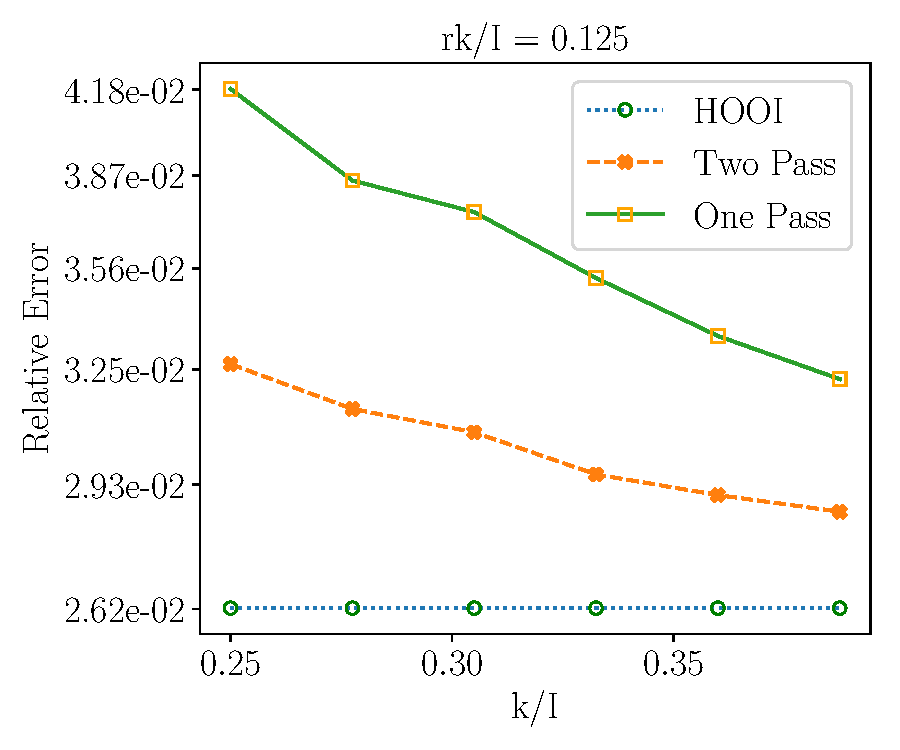
\includegraphics[scale = 0.3]{figure/SRFRAD_frk8.pdf}
    \end{subfigure}
    \begin{subfigure}{0.32\textwidth}
    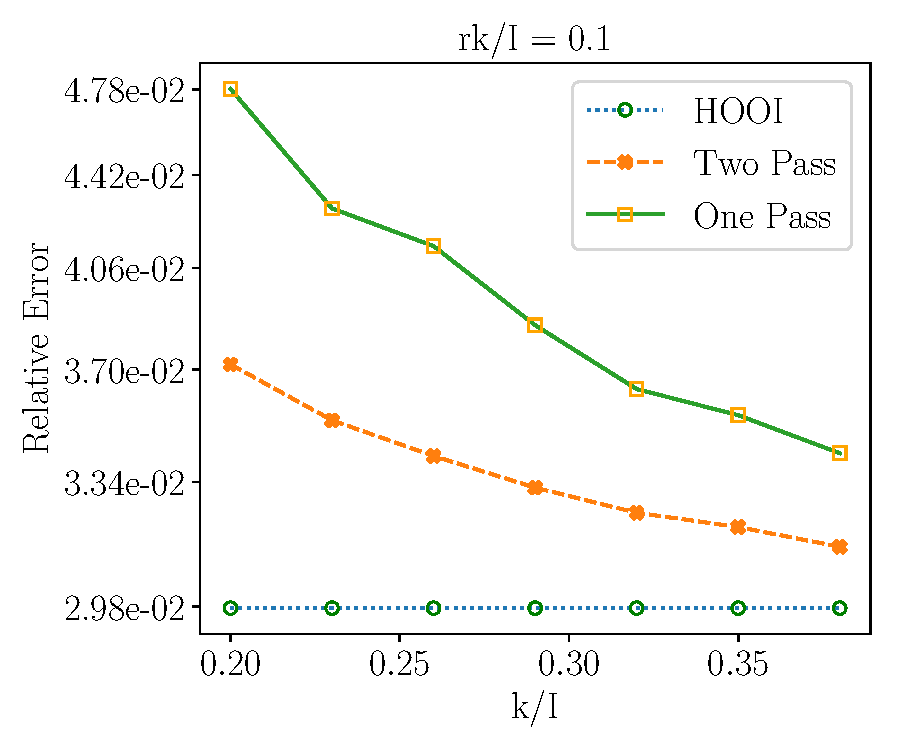
\includegraphics[scale = 0.3]{figure/SRFRAD_frk10.pdf}
    \end{subfigure}
    \begin{subfigure}{0.32\textwidth}
    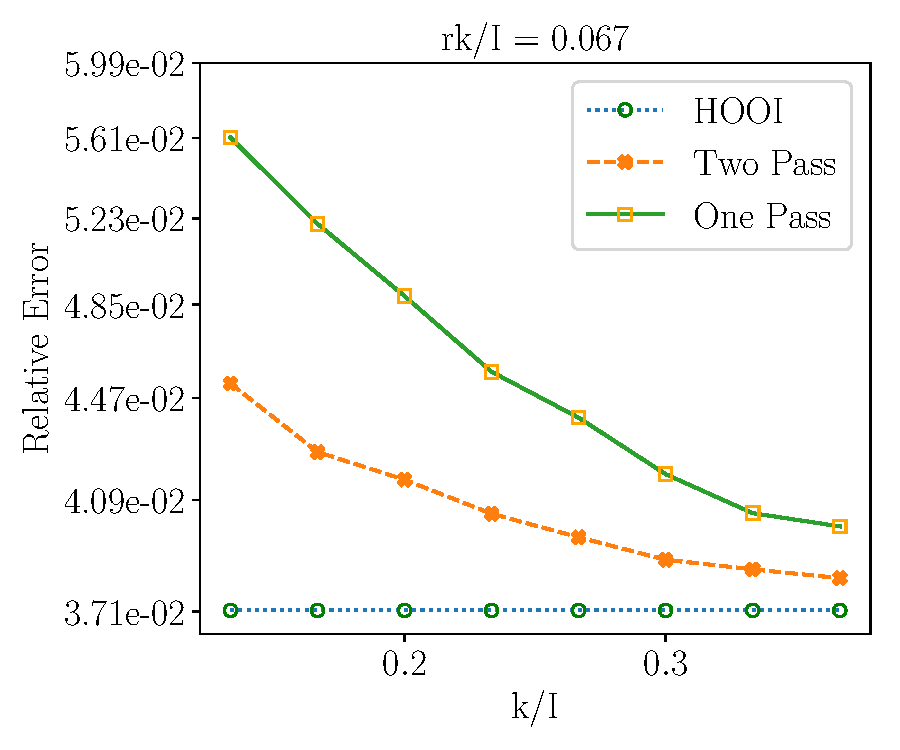
\includegraphics[scale = 0.3]{figure/SRFRAD_frk15.pdf}
    \end{subfigure}\\ 
    \textbf{Net Radiative Flux at Surface}
    \caption{Relative error for fixed-rank tensor approximation on the net radiative flux data ($1200 \times 192 \times 288$): \textit{We compare the relative errors presented in log scale for two-pass sketching, one-pass sketching and Tucker decomposition with different ranks ($rk/I = 0.125,0.2,0.067$). The dataset comes from the CESM CAM and the net radiative flux determines the energy received by the earth surface through radiation}} \label{fig:srfrad}
\end{figure}
\begin{figure}
    \centering
    \begin{subfigure}{0.32\textwidth}
    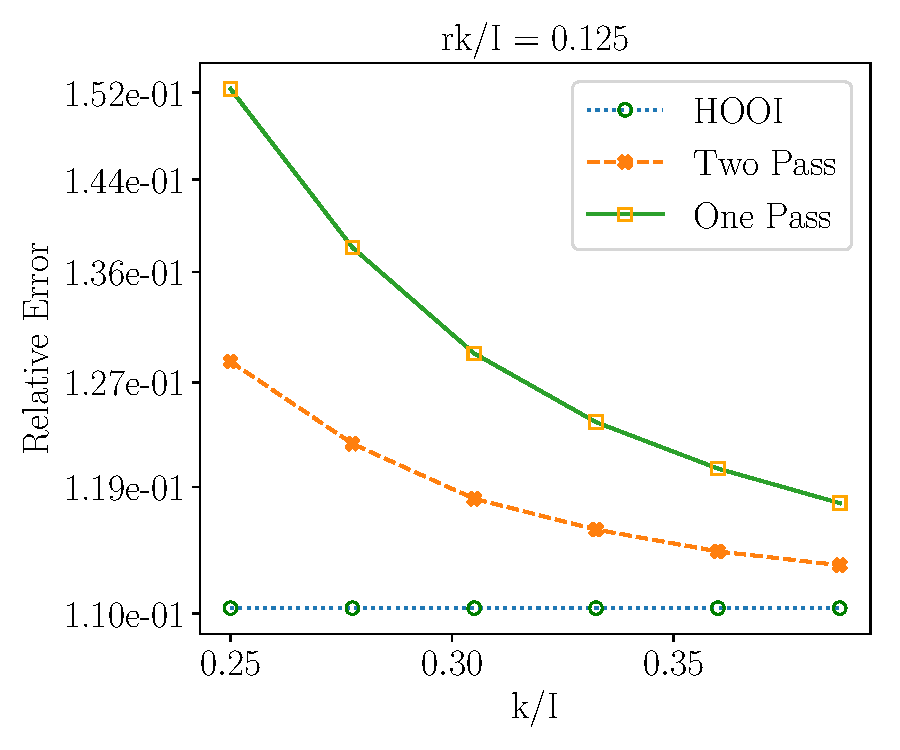
\includegraphics[scale = 0.3]{figure/BURDENDUST_frk8.pdf}
    \end{subfigure}
    \begin{subfigure}{0.32\textwidth}
    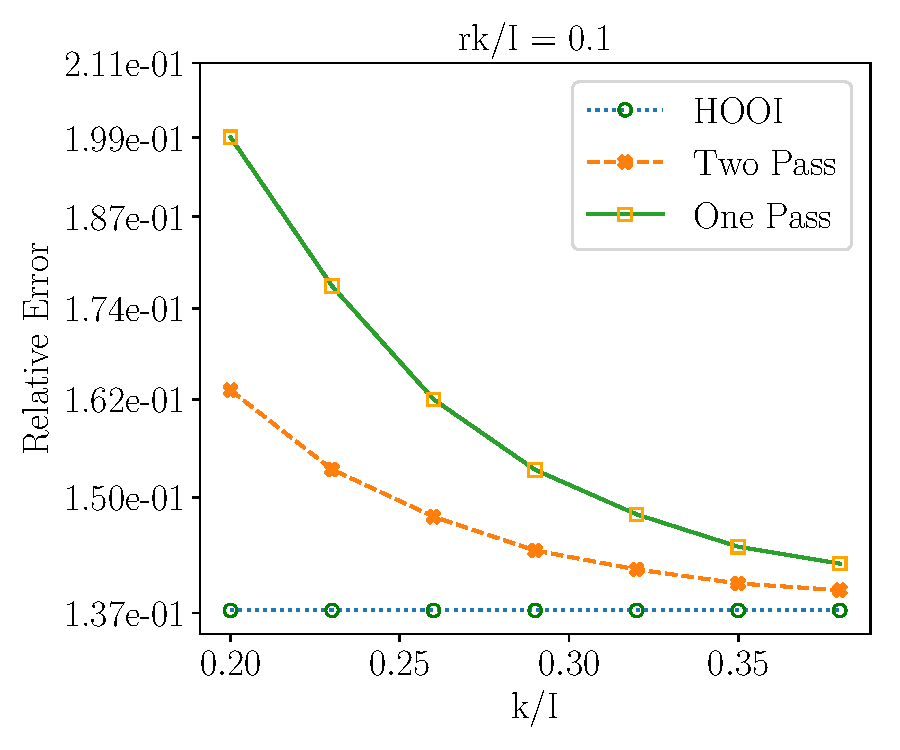
\includegraphics[scale = 0.3]{figure/BURDENDUST_frk10.pdf}
    \end{subfigure}
    \begin{subfigure}{0.32\textwidth}
    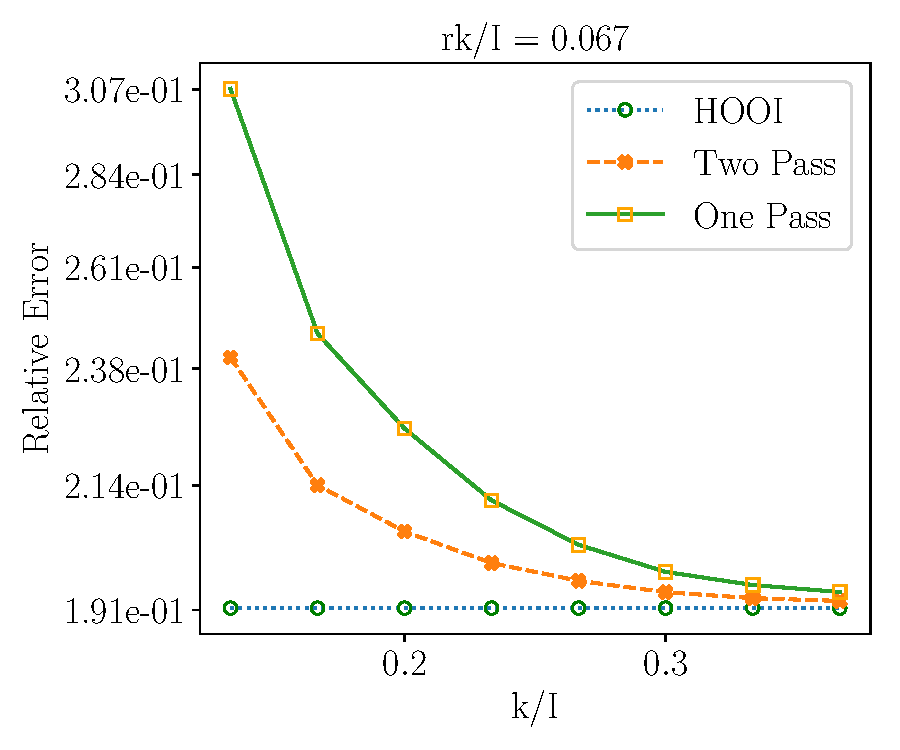
\includegraphics[scale = 0.3]{figure/BURDENDUST_frk15.pdf}
    \end{subfigure}
    \textbf{Dust Aerosol Burden}
    \caption{Relative error for fixed-rank tensor approximation on the dust aerosol burden data ($1200 \times 192 \times 288$): \textit{We compare the relative errors presented in log scale for two-pass sketching, one-pass sketching and Tucker decomposition with different ranks ($rk/I = 0.125,0.2,0.067$). The dataset comes from the CESM CAM and the dust aerosol burden measures the amount of aerosol contributed by the dust.}} \label{fig:burden_dust}
\end{figure}